\chapter{Introduction}
Smart environments are comprised of numerous sensing and computing devices. They support a number of users in this environment in performing their tasks. Driven by advances in computing power, miniaturization of sensors and processing methods, novel devices that have a plethora of functionality are introduced into our everyday lives. As a scientific field it has been thriving in the last decades. It combines knowledge from disciplines including computer science, engineering, or product design. Systems are  created that are integrated into the environment, have a high usability, and provide information and services to the actors in smart environments. Perhaps the most cited example of this trend is the rise of the smartphone, from professional business tool to a consumer device, being sold hundreds of millions times a year. Using integrated sensors and communication facilities it is possible to provide services aware of location, schedule, contacts, or preferences. They realize navigation, event planning, augmented reality, or entertainment. Another example is given by increasingly connected homes that are aware of energy usage, lighting levels, temperature and the status of critical devices. They can be controlled by the user from a single place or autonomously using a set of specified rules. 

A common aspect of all smart environments and smart devices is sensing. This includes environmental parameters, but also system state and most importantly the activities of the different users. There are numerous categories of sensing devices that can realize different aspects of this sensing, including cameras, accelerometers, GPS, or acoustic sensors. Capacitive sensors are a category of sensors that use electric fields to sense the presence and certain properties of the human body. The most common variety is sensing the presence of fingers on touch screens, which is already present in billions of devices. However, there is another variety, the capacitive proximity sensor. It is able to detect the presence of human body parts over a distance, providing interesting applications in smart environments. These are enabled by unobtrusively integrating the sensors into different materials, environments and appliances. When creating an application of smart environments choosing the right sensors is one of the most critical decisions that has to be taken early in the design process. Even though there are numerous prototypes available, so far this process has been mostly supported by looking at previous activities. 

In this work I present a benchmarking model that can support this decision process in the domain of smart environments. This allows to determine relevant application areas for capacitive proximity sensors. For each area there are different challenges that have to be considered, concerning the details of choosing hardware layout and suitable algorithms. I will present a collection of existing and novel methods that support processing data generated by capacitive proximity sensors. To evaluate the feasability of those methods, several prototypes have been created and tested for performance and usability. Figure \ref{fig:all_protos} shows sketches of the different prototypes and the placement of the electrodes attached to the capacitive proximity sensors. Based on these evaluations and the knowledge generated in the design process, I am able to discuss the benefits and limitations of the technology and classify it with regards to competing technologies. This allows me to present a set of guidelines that can aid parties interested in designing smart environment applications using capacitive proximity sensors.
 
\section{Motivation}
\begin{figure}[h]
\centering
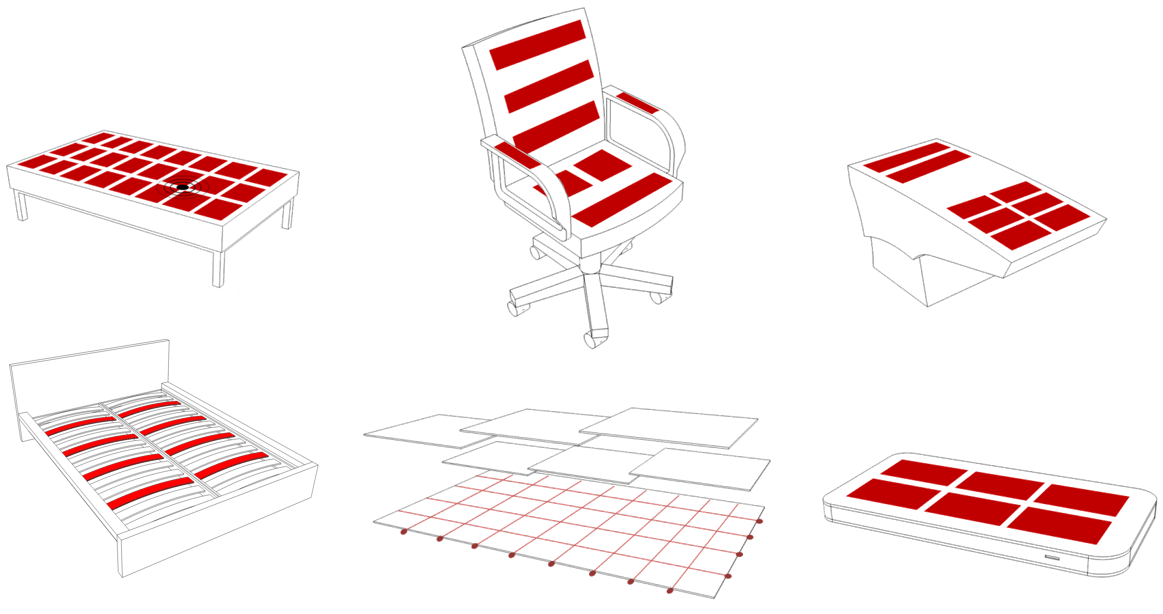
\includegraphics[width=0.9\textwidth]{images/all_protos}
\caption{Sketch of electrode placement of all capacitive sensing prototypes created in the scope of this work}
\label{fig:all_protos}
\end{figure}
In the last decade the way we interact with computing machines has changed in a profound fashion. Today more than one billion people operate a smartphone, enabling ubiquitous access to communication tools, processing power and information. The vision of ubiquitous Computing as proposed by Mark Weiser in the early 90s is moving closer to reality \cite{Weiser1991}. The required technologies of \begin{quote}
"cheap, low-power computers that include equally convenient displays, a network that ties them all together, and software systems implementing ubiquitous applications" 
\end{quote}
are now existing in the form of smartphones and tablets that are connected to the internet, using high-speed connections such as LTE (Long Term Evolution, also known as 4G - a high speed mobile communication protocol), and web-based services such as Google Now, that combine numerous data sources to provide personalized services.

While the vision and underlying ideas remain similar, alternative names for Ubiquitous Computing have been used in research, including Pervasive Computing and Ambient Intelligence. The concept has been expanded not only to consider devices that can be directly manipulated, but also include determining the current situation and can react based on it. This context-aware computing proposes 
\begin{quote}
"systems that examine and react to an individual's changing context. Such systems can promote and mediate people's interactions with devices, computers, and other people" \cite{schilit1994context} 
\end{quote}
Different forms of context can be distinguished, ranging from location and the actual system state, to different activities or even the current mood of the user. In order to acquire this context, the input-and-output based systems originally proposed by Weiser are augmented by an ensemble of devices that are very small (dust), coordinate in massive numbers (clay), or are flexible, unobtrusive extensions to everyday objects (fabric) \cite{poslad2011ubiquitous}. These devices can be invisibly integrated into our everyday environment and provide sensing capabilities that can be used by systems that are sufficiently small. Examples of these devices are microelectromechanical systems (MEMS) or mechanically flexible electronics, such as OLED screens. The number of computation and sensing devices that we carry with us is growing continuously. Yet we want the technology to further disappear, allowing us to focus on the application instead of the underlying technology. 

The famous science fiction author Arthur C. Clarke proposed three laws of prediction, the third of which is 
\begin{quote}
"Any sufficiently advanced technology is indistinguishable from magic." \cite{clarke1962hazards} 
\end{quote}
Capacitive proximity sensing allows us to measure the influence of the human body (or conductive objects in general) on an electric field. While this technology is not magic per se, a peculiarity of electricity is that humans, as opposed to some animals, have no specific sensing organs for this property. Thus we remain unaware of their presence, unless the field strength is very high, leading to electric shocks. Consequently, when interacting with capacitive sensors there is no awareness of what they are sensing unless it is specifically exposed to another sense of the user. This could be haptic feedback on touch screens or visual feedback on free air interaction systems. Touch screens are the most ubiquitous application of capacitive technology. It is applied in all modern smartphones and tablets, thus being used by a large number of the world's population every day. However, they are typically tuned to only register touches, with some varieties being able to detect objects over a small distance. This enables numerous other applications for this technology, ranging from industrial fluid level and material detection, to presence detection in cars. A particularly interesting domain for this sensing technology is smart environments. As previously mentioned they provide services based on unobtrusively acquired information about persons currently acting in this environment. In this regard they can be considered as part of the fabric - unobtrusive extensions to everyday objects. Capacitive proximity sensors have been primarily used for human-computer interaction (HCI) applications, including a mouse tracking the distance of the heel of the hand, or a monitor that is able to track gestures performed in front of it. Another application are smart appliances, such as an object detecting car seat or localization systems. 

In smart environments there are numerous sensing technologies that provide similar detection capabilities. Looking at the recognition of simple activities, such as standing, walking and lying, cameras and accelerometers can lead to the same result. Thus, it is often difficult to decide what the specific sensor technology to use in a specific system. Commonly, one refers to previous work and best practice, building on previously generated knowledge. However, so far there is no formal model that would allow to quickly evaluate different sensor technologies for different applications. Taking into account a specific set of features required for a specific application domain this could be an important decision support tool in the early stages of system development. As it was stated by Cook and Das \cite{cook2007smart}:
\begin{quote}
"Finally, a useful goal for the smart environment research community is to define evaluation mechanisms. While performance measures can be defined for each technology within the architecture hierarchy [...], performance measures for entire smart environments still need to be established. This can form the basis of comparative assessments and identify areas that need further investigation."
\end{quote}
Such a tool can also be used to identify specific applications for a single sensor technology, such as verifying current and developing new use cases for capacitive proximity sensors or providing a classification of the technology with regards to competing sensor systems. However, identifying a suitable sensor is just the first step in designing a smart environment prototype or product. After this decision a designer has to determine specific challenges of the domain, select suitable methods for applying the technology and processing the data and create a working system. In this design step it is helpful to have a set of methods, examples and guidelines, leading to a more rapid prototyping for researchers and shorter time-to-market for product developers. These guidelines should be the result of literature review and validating prototypes for performance and usability. 

\section{Research Challenges}
There have been numerous influential works that gave an overview of technologies and applications in smart environments. Cook and Das identified common technologies, frameworks and applications in this domain and gave an overview of ongoing research \cite{cook2007smart}. Poslad specified a more detailed taxonomy of device classes, provided concepts for interaction between humans and environments and gave an overview of intelligent systems \cite{poslad2011ubiquitous}. A different category of previous work details the different sensing technologies that are supporting various different applications and provided an overview of limitations and benefits. However, so far there has been no work that provides a benchmark that maps different sensor characteristics to applications in smart environments. An intermediate step between evaluating entire environments and low-level technologies is an application-specific benchmarking of systems. Benchmarking as a method allows us to quantify the performance of a specific process or item and thus allows a comparison to similar entities. It is common to benchmark different technologies according to their features. I therefore propose to extend technology-driven benchmarks by adding an application-specific feature weighting. This approach will be introduced in Chapter \ref{ch:benchmark}. It allows to map the same set of features to different applications that have similar requirements, which can be realized by multiple technologies. It will be verified by benchmarking typical applications with regards to several example applications in the domain of smart environments.

The selection of application scenarios for capacitive proximity sensors is mostly driven by previous work, most notably by research groups from MIT \cite{Zimmerman1995}, Disney research \cite{Sato2012} and the Munich University of Technology \cite{Wimmer2006}. They are extending on the methods or modify existing use cases to another domain. A more formal approach might allow to verify existing use cases, enable a comparison with other sensing technologies, or even find novel applications for capacitive proximity sensors. I propose using the developed benchmarking method for this purpose, as shown in Chapter \ref{ch:benchmark_applications}. This way it is possible to verify the existing application areas or even determine new ones. Additionally, one can specify if other sensing technologies might be more suitable for a specific application. This allows me to identify four relevant application domains that can be realized with capacitive proximity sensors. 

Following the design process, a next step is specifying the particular challenges for the given application. This allows selecting suitable processing methods, in order to create and evaluate the system. Looking at the related works several areas are identified that can be improved using novel or adapted methods. E.g. previous systems often rely on uniform sensor arrays \cite{Smith1996a} or require a large number of sensors \cite{rekimoto2002smartskin}. I propose improvements to five different areas in Chapter \ref{ch:prot_proc}. These are object tracking using a restricted sensor count, model-driven approaches for object fitting, heterogeneous sensor systems, image-based processing of capacitive sensor data, and physiological sensing. The presented methods are realized in different prototypes that are evaluated for usability and performance, as detailed in Chapter \ref{ch:usecases}.

While there are numerous applications based on capacitive proximity sensors, there has been no distinct classification within smart environments. This should include a comparison to other sensor technologies, as well as identifying benefits and limitations for capacitive proximity sensors. Using the knowledge generated from determining applications, their specific challenges and creating different prototypes I am able to classify capacitive proximity sensors with regards to other sensing technologies in the domain of smart environments. This is shown in Chapter \ref{ch:eval}. It is possible to identify specific benefits and limitations and compare features between technologies. This culminates in creating a set of guidelines for parties that are interested in developing smart environment systems based on capacitive proximity sensors.
 
\section{Contributions}
In the following I will briefly list the specific contributions provided by this work on a methodological and practical level. They are separated into three different groups: the benchmarking model, the introduction of new or improved processing methods, and the classification validation of capacitive proximity sensors within smart environments.
\begin{enumerate}
\item \emph{Introduction of a generic and formal benchmarking model for sensor systems in smart environments} 

This allows to create or verify use cases for any given sensor technology in smart environments. For this purpose, I will identify the most relevant sensor features for the scoring process, create a feature matrix that links features to application importance rating. Additionally, the benchmarking score calculation, including normalization and compensation for central-tendency bias, will be specified. The method is applied to capacitive proximity sensors to find and verify use cases.
%\begin{itemize}
%\item Identification of relevant sensor features to be included in the scoring process
%\item Feature matrix linking features to application importance ratings
%\item Benchmark score calculation including methods for normalization and avoiding central-tendency bias
%\item Determining suitable use cases for capacitive proximity sensors in smart environments
%\end{itemize} 
\item \emph{New and improved processing methods for capacitive proximity sensors} 

Based on the specified use cases, a set of associated challenges can be generated that leads to potential areas that require new and improved processing methods. For sparse sensor distributions I developed a new method allowing indoor localization and fall detection, as well as new approaches for hand tracking. I propose two novel methods for model-driven processing to detect occupation and pose with both single-body models and multi-body models. Looking at heterogeneous sensor system, I investigate methods to handle non-uniform arrays and provide an integration of capacitive proximity sensors and acoustic systems. I introduce a new method for image-based processing of capacitive sensor data from uniform arrays, allowing tracking of multiple objects in three dimensions. Finally, two methods for tracking physiological activities are introduced that operate in time- and frequency-domain. They can be used to detect the sleep phase or respiratory rate.
%These are grouped into methods 
%realizing the use cases specified 
%\begin{itemize}
%\item Identification of challenges associated to all use cases
%\item Processing methods for sparse sensor distributions improving localization and fall detection, as well as hand gesture recognition
%\item Model-driven processing methods for single and multi-body models used for occupation and pose recognition of persons
%\item Methods for processing in heterogeneous sensor systems comprised of non-uniform array configurations, parallel processing of single data streams or fusion of different sensor systems
%\item Considerations regarding image-based processing for loading mode sensors in uniform array configurations
%\item Several methods to process physiological signals using different sensing modes in frequency- and time-domain. 
%\end{itemize}
\item \emph{Proof-of-concept and evaluation of processing methods using a variety of prototypes}

The \emph{MagicBox} enables expressive single-hand gestural interaction with sparse sensor distribution and machine learning gesture classification. \emph{CapFloor} proposes a novel layout for floor-based capacitive indoor localization systems, enabling unobtrusive application, easy maintenance and fall detection. The \emph{SmartBed} uses a model-based approach for fitting one or two persons, concurrently detecting sleep phases and breathing rate for one occupant.
The \emph{Capacitive Chair} is a piece of smart furniture that allows to detect presence, identify users, track different postures, measure breathing rate and enables novel applications for smart offices. A heterogeneous sensor layout to enable different forms of interaction in automotive environments is implemented in the \emph{Active Armrest}. The \emph{CapTap} combines capacitive sensors and microphones in a table-based interaction device, enabling multi-hand gesture recognition in three dimensions using an interaction pattern of multiple layers.
%\end{description}

%\begin{description}
%\item[MagicBox] Enabling expressive single-hand gestural interaction with sparse sensor distribution and machine learning gesture classification
%\item[CapFloor] Novel layout for floor-based capacitive indoor localization systems, enabling unobtrusive application, easy maintenance and fall detection
%\item[SmartBed] Model-based approach for fitting one or two persons, concurrently detecting sleep phases and breathing rate for one occupant
%\item[Capacitive Chair] Smart furniture that allows to detect presence, identify users, track different postures, measure breathing rate and enables novel applications for smart offices
%\item[Active Armrest] Heterogeneous sensor layout to enable different forms of interaction in automotive environments
%\item[CapTap] Combining capacitive sensors and microphones in a table-based interaction device, enabling multi-hand gesture recognition in three dimensions using a multi-level interaction pattern
%\end{description}
%\end{itemize}
%Determine suitable use cases for capacitive proximity sensors in smart environmIn order to validate the sensor technology different challenges are determined for each use case, allowing to identify processing methods that can be beneficial. Processing methods in five different groups are presented. Two methods for sparse sensor configurations that enable tracking hand gestures in three dimensions and localization and fall detection in large areas. Several model-driven fitting methods applying machine learning on single- and multi-body models.. Considerations regarding image-based processing for loading mode sensors in uniform array configurations. Several methods to process physiological signals using different sensing modes in frequency- and time-domain.
\item \emph{Classification of capacitive proximity sensors in smart environments}

Based on the knowledge gathered in analyzing the existing works and creating the number of prototypes I am able to provide a classification of capacitive systems. The first step is a comparison to other sensor technologies that are commonly used in smart environments. I will establish benefits and limitations for capacitive proximity sensors in comparison to competing sensing systems. This leads to the creation of a set of guidelines that support designers interested in creating smart environment applications based on capacitive proximity sensors.
%\end{itemize}
%Six different prototypes are detailed and evaluated. The MagicBox prototype, enabling expressive single-hand gestural interaction with sparse sensor distribution and machine learning gesture classification. The CapFloor system, using a novel layout for floor-based capacitive indoor localization systems, enabling unobtrusive application, easy maintenance and additional services such as fall detection. The SmartBed prototype using a model-based approach for fitting one or two persons, concurrently detecting sleep phases and breathing rate for occupants. The Capacitive Chair smart furniture that allows to detect presence, identify users, track different postures, measure breathing rate and enables novel applications for smart offices. The Active Armrest using a heterogeneous sensor layout to enable different forms of interaction in automotive environments. The CapTap prototype combining capacitive sensors and microphones in a table-based interaction device, enabling multi-hand gesture recognition in three dimensions using a multi-level interaction pattern. Three other prototypes, CapDisp, HoneyFish and GestDisp, that were created in collaborative efforts are described briefly.
\end{enumerate}

%\item Image-based processing methods for loading mode sensors
%\item Processing of physiological signals in frequency- and time domain
%\begin{itemize}
%\item Benchmarking model for sensors in smart environments
%\begin{itemize}
%\item Identification of application domains in smart environments
%\item Application-centric benchmarking model for mapping a single set of sensor features to different smart environment applications
%\item Identification of applications suitable for capacitive proximity sensors based on the developed benchmarking model
%\end{itemize}
%\item Validation of capacitive proximity sensors in smart environments
%\begin{itemize}
%\item Specifying challenges in the presented application domains
%\item Improved processing methods related to these challenges
%\begin{itemize}
%\item Processing methods for sparsely distributed sensor arrays including 3D hand tracking and large-area localization
%\item Model-driven fitting methods using machine-learning methods on single-, and multi-body models
%\item Heterogeneous sensor systems comprised of non-uniform array configurations, parallel processing of single data streams and fusion of different sensor systems
%\item Image-based processing methods for loading mode sensors
%\item Processing of physiological signals in frequency- and time domain
%\end{itemize}
%\item Application prototypes
%\begin{itemize}
%\item MagicBox prototype enabling expressive single-hand gestural interaction with sparse sensor distribution and machine learning gesture classification
%\item CapFloor prototype using a novel layout for floor-based capacitive indoor localization systems, enabling unobtrusive application, easy maintenance and additional services such as fall detection
%\item SmartBed prototype using a model-based approach for fitting one or two persons, concurrently detecting sleep phases and breathing rate for occupants
%\item Capacitive Chair prototype that uses allows to detect presence, identify users, track different postures, measure breathing rate and enables novel applications for smart offices
%\item Active Armrest prototype uses a heterogeneous sensor layout to enable different forms of interaction in automotive environments
%\item CapTap prototype combining capacitive sensors and microphones in a table-based interaction device, enabling multi-hand interaction in three dimensions using a multi-level interaction pattern
%\item Short description of CapDisp, Honeyfish, GestDisp
%\end{itemize}
%\item Discussion of limitations and benefits of capacitive proximity sensors in smart environments and comparison to other sensing technologies
%\end{itemize}
%\item Interaction and localization in smart environments
%\begin{itemize}
%\item Marker-free interaction with arbitrary devices in smart environments
%\item Presentation of AmbiTrack - a camera-based indoor localization system for smart environments
%\end{itemize}
%\end{itemize}

\section{Structure of this work}
The relevant literature is specified in Chapter \ref{ch:related_work} - \emph{\nameref{ch:related_work}}. It is grouped into four categories. The first section gives a background on electric field sensing, including relevant historical work and the physical properties. Additional different sensing categories are outlined, before different electrode considerations and data processing methods are introduced. The second category of related works discusses different applications of capacitive proximity sensors that were created in the last decades, ranging from MIT research in the early 90s, to novel touch classifiers based on different sensing methods. The third category introduces different competing technologies that will be used in the later benchmarking. Finally we give an overview of existing work collecting and grouping applications in smart environments. This will allow us to identify candidate scenarios for capacitive proximity sensors.

Chapter \ref{ch:benchmark} - \emph{\nameref{ch:benchmark}} - is introducing the application-specific benchmarking model. In the first part of this chapter the sensor features relevant for application in smart environments are discussed. Suitable features are discussed in three different categories, discussing the rationale for inclusion or omission in the model. The next part describes the benchmarking model. The application-based feature weighting is introduced, leading to the derivation of the model itself, including the required calculation of an overall rating and a feature score normalization. After that we are using the model to score different examples and validate those using search results from scientific publication databases. Afterwards, the model is discussed and used to identify suitable applications for capacitive proximity sensors in smart environments.

Chapter \ref{ch:usecases} - \emph{\nameref{ch:usecases}} - outlines the previously identified use cases. First, the  associated challenges for design and processing are identified. Afterwards, different processing methods for capacitive proximity sensors are presented that tackle the specific challenges. This includes methods for sparsely distributed sensor arrays, model-based data fitting, heterogeneous sensor systems, image-based processing and physiological signal processing. Six different prototypes that implement one or more of the processing methods are presented and evaluated - MagicBox, CapFloor, Capacitive Chair,  Active Armrest, SmartBed and CapTap. Each of the prototypes has been evaluated for performance and usability. Additionally, three other prototypes are discussed briefly.

The knowledge gathered in designing, building and testing the prototypes leads to Chapter \ref{ch:eval} - \emph{\nameref{ch:eval}}, wherein the results are discussed and evaluated. This chapter has four parts. At first, capacitive proximity sensors are compared to the other sensor classes introduced in the related works. Afterwards, limitations and benefits of the technology are collected and linked to sensor features and applications. The chapter concludes with a set of guidelines that may help interested parties in evaluating their application for usage with capacitive proximity sensors and give practical help when applying this technology.

The document concludes in Chapter \ref{ch:conclusion} - \emph{\nameref{ch:conclusion}} - that briefly recapitulates the work and introduces potential future research based on this work.

There are four different appendices. Appendix A includes raw results and additional material of the evaluations performed with the different prototypes. Appendix B lists publications and talks. Appendix C lists Master and Bachelor Thesis that were supervised or co-supervised. Appendix D contains a short CV.